\RequirePackage{fix-cm}
\documentclass[smallextended]{svjour3}       % onecolumn (second format)
\usepackage[cp1250]{inputenc}
\usepackage{amsmath}
\usepackage{bbm}
\usepackage{color}

\newtheorem{df}{Definition}

\usepackage{graphicx}


\bibliographystyle{spmpsci}
\usepackage[numbers,square,sort&compress]{natbib}


\begin{document}

\title{Combination of Kolmogorov-Smirnov statistic and time-frequency representation for P-wave arrival detection in seismic signal.}
%\subtitle{Do you have a subtitle?\\ If so, write it here}

\titlerunning{KS statistic and time-frequency representation for seismic P-wave detection}        % if too long for running head


 \author{%
 Jacek Wodecki, Anna Michalak, Pawe{\l} Stefaniak, Agnieszka Wy{\l}oma{\'n}ska, Rados{\l}aw Zimroz
}%


\institute{ Jacek Wodecki \and Anna Michalak \and Agnieszka Wy{\l}oma{\'n}ska \and Pawe{\l} Stefaniak  
\at KGHM Cuprum Ltd, Research and Development Centre, Sikorskiego 2-8, 53-659 Wroclaw, Poland \and
Rados{\l}aw Zimroz
\at Faculty of Geoengineering, Mining and Geology, Wroclaw University of Science and Technology,  Na Grobli 15, 50-421 Wroclaw, Poland}

\authorrunning{Jacek Wodecki et al.} % if too long for running head

\date{Received: date / Accepted: date}

\maketitle

\begin{abstract}
The problem of determination of P-wave onset moment is elementary in seismic signals analysis. This problem is also widely discussed in the literature. In recent years many methods based on statistical properties of the signal have arisen. From the mathematical perspective the problem reduces to segmentation of the raw signal into parts with different features. Having the knowledge of the particular P-wave onset moment (for couple differently located sensors), the establishment of corresponding event's location and energy is possible. The difference in signals' frequency spectra for the registered event and its preceding noise allows for using time-frequency domain in designating the onset moment. In this paper an innovative method for searching of the P-wave arrival is proposed. The method incorporates using signal's time-frequency representation (namely spectrogram) and Kolmogorov-Smirnov (KS) statistic analysis. We apply two-sample one-sided Kolmogorov-Smirnov statistic to spectra vectors obtained from the spectrogram. On the basis of KS map it is possible to find the regime switching point which indicates the P-wave onset moment. The method is tested on a real life signal originating from underground mine. Proposed methodology is compared with classical Short-Time Average over Long-Time Average (STA/LTA) algorithm and P-wave arrival moment indicated manually by the expert.

\keywords{Kolmogorov-Smirnov statistic, P-wave detection, seismic data}
\end{abstract}

\section{Introduction}

One of the most crucial challenges in terms of seismic activity monitoring is recognition of seismic wave onset moment. Identification of this particular point in time leads to assessment of basic properties for registered event, i.e. its location, energy etc. \cite{kwiatek2013assessment}. These attributes are fundamental from view point of further seismic hazard assessment. Data acquisition system is used for monitoring of rock mass activity. This data should be next evaluated and interpreted (information about energy and localization of the event is required). In typical deep mine one could expect dozens of events per day. In practice this task is technically very difficult and complex, and daily will require extensive analysis of hundreds of signals from multiple different data receivers distributed spatially in wide area. Each signal should be interpreted immediately after measuring. Therefore it is recommended that such procedures for marking the P-wave onset moment should be automatic. In the literature this subject has been widely studied, however still the most commonly used technique is (STA/LTA) for preliminary detection, which is often corrected manually. When considering seismic signal which includes pure noise at the beginning (which is most commonly regarded as white) and actual seismic event subsequently, it is easy to denote a point in which the signal loses its stationary character. This is a consequence of occurrence of sudden instantaneous energy growth which is visible in the signal in form of amplitude variation increase. When considering time-frequency domain, sole change of signal power will be visible in spectrogram (due to Parseval's theorem). During P-wave onset moment the frequencies amplitudes rise as well as their proportions, so the short-time spectrum becomes much more non-uniform. The pure noise spectrum is flat and recorded seismic event has relatively wide frequency range at first, which is becoming narrower in time. Existing algorithms include STA/LTA, AR-based algorithms (finding different models for both event parts and a noise one \cite{sleeman1999robust,leonard1999multi}), algorithms using neural networks \cite{wang1995artificial}, or multiscale wavelet analysis \cite{zhang2003automatic}. The reader is referred to \cite{leonard2000comparison,withers1998comparison}, where the comparison of some classical algorithms has been investigated. The recent work on this subject includes \cite{sokolowski2016algorithm,nurhaida2017detecting,polak2017seismic,zimroz20150000}, and their comparison can be found in \cite{sokolowski2016comparison}. First mentioned group of algorithms is based mainly on sole time domain and ignores capability of frequency domain. The potential hidden in time-frequency domain has been presented in \cite{hafez2009earthquake,xiantai2011adaptive}. Effectiveness of these methods confirms an adequacy of using the spectrogram in term of finding P-wave onset moment. Hence, development of method based on spectrogram in P-wave recognition is justified.

Authors propose to analyze spectrogram of seismic signal using Kolmogorov-Smirnov statistic values arranged into a map \cite{wodecki2017technical}. In presented approach it is used to differentiate the structure of spectra vectors from the spectrogram. This enables the separation of spectra vectors from before and after the arrival moment. As a result we can determine arrival moment as a point located between obtained groups of spectra vectors. Such approach is fully data-driven in its analytical process. 


\section{Methodology}

In this section the overall methodology is explained (see Fig. \ref{fig: block}).

\begin{figure}[!ht]
\centering
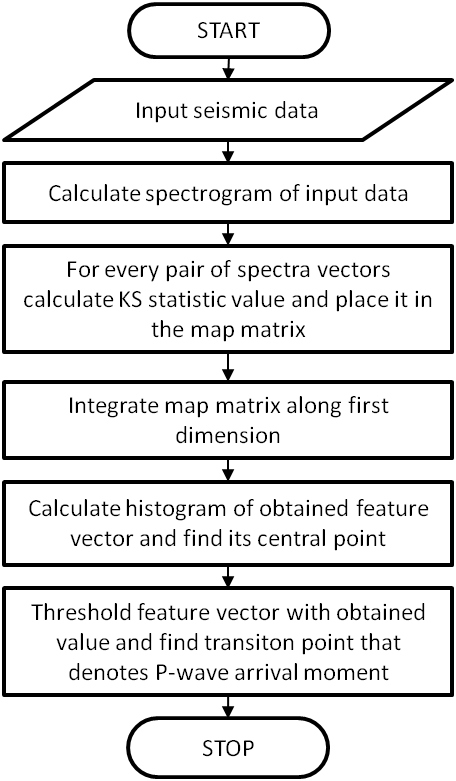
\includegraphics[width = 0.45\textwidth]{figs/block}
\caption{Flowchart of presented procedure}
\label{fig: block}
\end{figure}


Presented procedure begins with calculating spectrogram (see Equations \ref{eq:spectrogram} and \ref{eq:spec}). Its parameters are selected based on empirical testing and are suited best for the length of signal time series, in relation to the way that prior segmentation algorithm selects and segments the individual seismic events. For analyzed signal the parameters are presented in Table \ref{tab:tab}.

The short-time Fourier transform (STFT) for the discrete signal\\ $x_0, x_2, \dots , x_{N-1}$ is defined as follows \cite{oppenheim1999discrete}:
\begin{equation}
\label{eq:spectrogram}
\textrm{STFT}(t,f)=\sum_{m=0}^{L-1} x_{t+m}\omega_{m}e^{-j2\pi fm/N}
\end{equation}
for $0\leq f\leq f_{max}$ and $0\leq t\leq t_{max}$. In the above equation $\omega$ is the shifted window of the length $L$. Furthermore, the spectrogram is squared absolute value of the STFT:

\begin{equation}
\label{eq:spec}
\textrm{Spec}(t,f)=|\textrm{STFT}(t,f)|^2.
\end{equation}


After that, for each non-repeating pair of spectra vectors, the Kolmogorov-Smirnov (KS) statistic is calculated (see Definition \ref{def}).

\begin{df}[Kolmogorov-Smirnov statistic]\label{def}

The two-sample one-sided Kolmogorov-Smirnov (KS) statistic for samples $y^1_1,y^1_2,\dots,y^1_K$ and $y^2_1,y_2^2,\dots,y^2_K$ of lengths $K$ is given by following formula:
\begin{equation}\label{def1}
    D^*_{1,2}=\max_{v}\left( \hat{F}_{y^1}(v)-\hat{F}_{y^2}(v) \right),
\end{equation}
where $\hat{F}_{y^i}(v)$ is empirical cumulative distribution functions of vector $y^{i}$, $i=1,2$ in point $v$ \cite{wang2003evaluating,massey1951kolmogorov}. 
\end{df}
In formula (\ref{def1}) the empirical cumulative distribution function for sample  $y_1, y_2, \dots, y_K$ is defined as follows:
\begin{equation}
    \hat{F}(v)= \frac{1}{K}\sum^K_{k=1}\mathbbm{1}_{\{ v_k\leq v\}},
\end{equation}
where $\mathbbm{1}_A$ is an indicator of a set $A$.

In our methodology we apply the KS statistic to spectra vectors taken  from the spectrogram. More precisely,  for all $i,j\in \{0,...,t_{max}\}$ we calculate  the value of KS statistic. All of obtained values $D^*_{i,j}$ are arranged into upper-triangular part of a square matrix $KS$, such as:
\begin{equation}
    KS_{(i,j)}=D^*_{i,j},\quad i=0,\dots,t_{max}, \quad j=i,\dots,t_{max},
\end{equation}
that is reflected with respect to the main diagonal in order to obtain symmetric matrix. Then, such matrix is integrated along one dimension producing a feature vector, which is then thresholded using central point of the histogram. It is performed by dividing spectrogram into two halves according to the item count, then finding two global modes as global maxima in each half of spectrogram, and finally defining central point as an average between modes. Threshold allows to automatically indicate the transition point between the processes (see section \ref{ks}).


\subsection{KS map and its interpretation}\label{ks}

\begin{figure}[!ht]
\centering
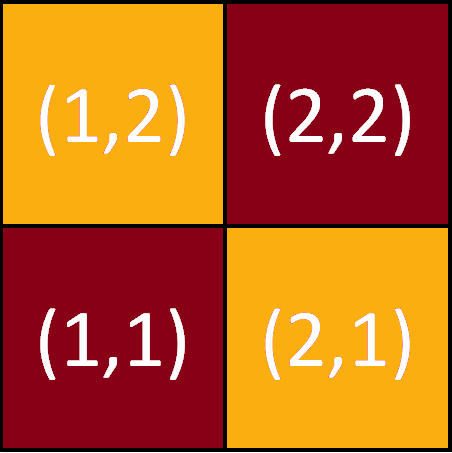
\includegraphics[width = 0.3\textwidth]{figs/mapc}
\caption{Conceptual chart of expected KS map}
\label{fig: mapc}
\end{figure}

Based on initial visual evaluation of the input data one can notice two disjoint processes occurring consecutively:

\begin{itemize}
\item \textbf{Process 1:} No seismic shocks are present, signal can be considered as a a noise (area (1,1));
\item \textbf{Process 2:} Seismic event occurs, signal presents the impact and its dampening (area (2,2)).
\end{itemize}

In such case one can describe those processes in terms of signal parameters:

\begin{itemize}
\item \textbf{Process 1:} Low energy, uniform spectrum;
\item \textbf{Process 2:} High energy, non-uniform and time-varying spectrum;
\end{itemize}


Despite the relatively good visibility of the events in the input data, it is not easy to define one simple, effective and precise evaluation criterion. Thus, proposed methodology is based on the analysis of the map constructed by composing the values of KS statistic. 

\section{Results}
Raw input signal of considered seismic event is presented in Fig. \ref{fig: raw}. In the first step spectrogram of the signal was calculated according to parameters in Table \ref{tab:tab} (see Fig. \ref{fig: spec}). 
\begin{table}[ht!]
    \centering
    \caption{Parameters of compared results}
  \begin{tabular}{|l|l|}
    \hline
    \textbf{Parameter} & \textbf{Value} \\ \hline
         Sampling frequency & 500 Hz \\ \hline
         Window & Hamming, 32 samples \\ \hline
         Overlap & $0.95\%$ \\ \hline
         FFT points & 256 \\
    \hline
    \end{tabular}
    \label{tab:tab}
\end{table}

\begin{figure}[ht!]
\centering
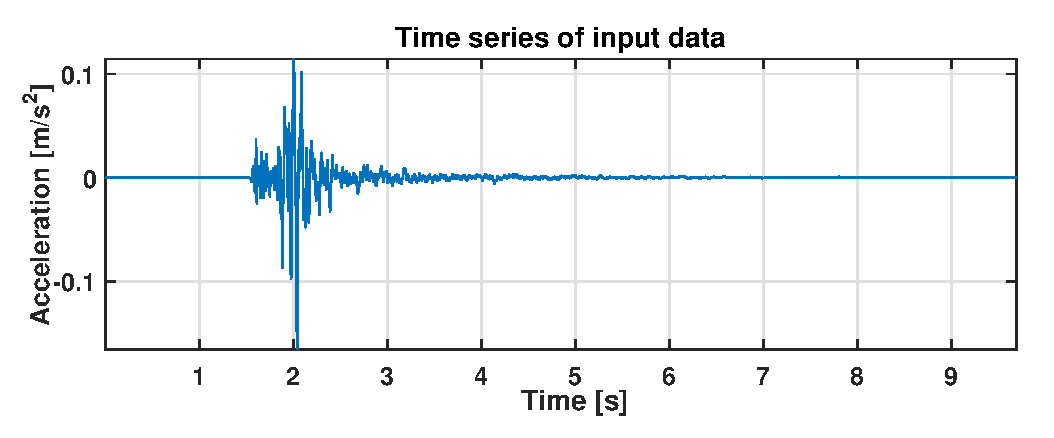
\includegraphics[width =0.8\textwidth]{figs/raw}%grafika do podmiany - proponuję ([-0.2 0.2])
\caption{Raw signal of seismic data}
\label{fig: raw}
\end{figure}

After that, individual spectra vectors are compared with each other in a non-repeating manner, and KS statistic produced by each comparison is placed in a upper-triangular half of a square matrix. It is then reflected to form a symmetric square matrix, which is further called a map. 



\begin{figure}[!ht]
\centering
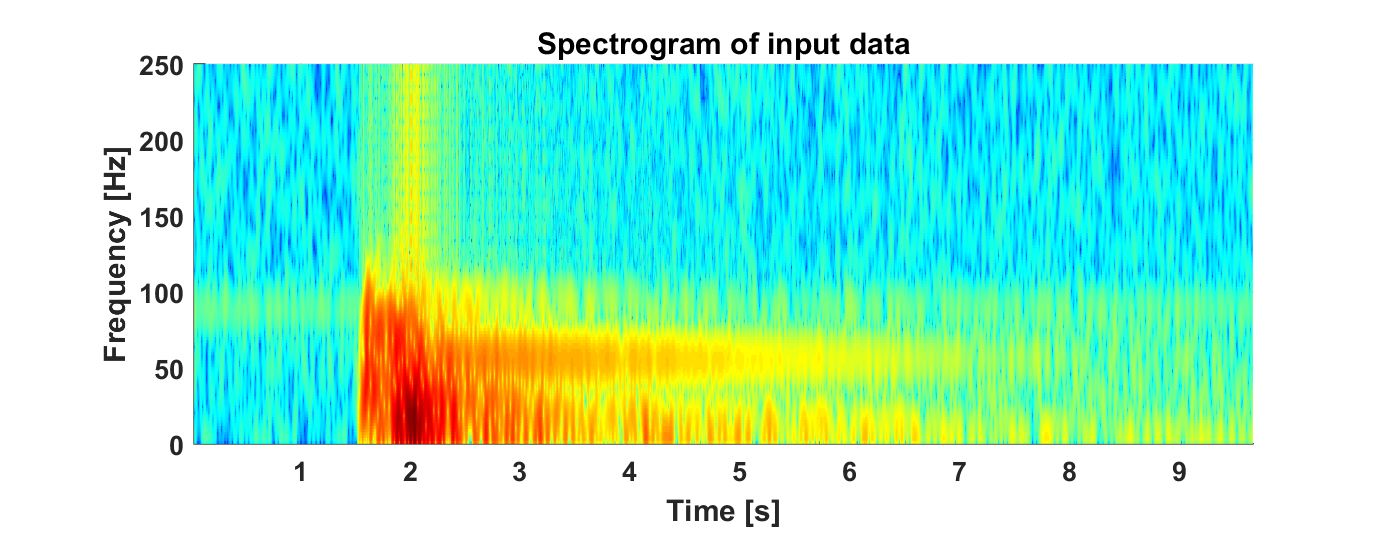
\includegraphics[width = 0.98\textwidth]{figs/spec}
\caption{Spectrogram of seismic data}
\label{fig: spec}
\end{figure}



It is hard to find transition points based on two-dimensional data. Hence, we propose to determine threshold based on one-dimensional statistic. Taking advantage of previously mentioned assumptions (see section \ref{ks}), it is expected that local sum of KS map vectors will vary according to the area (see Fig. \ref{fig: mapc}, \ref{fig: map}). 

\begin{figure}[!ht]
\centering
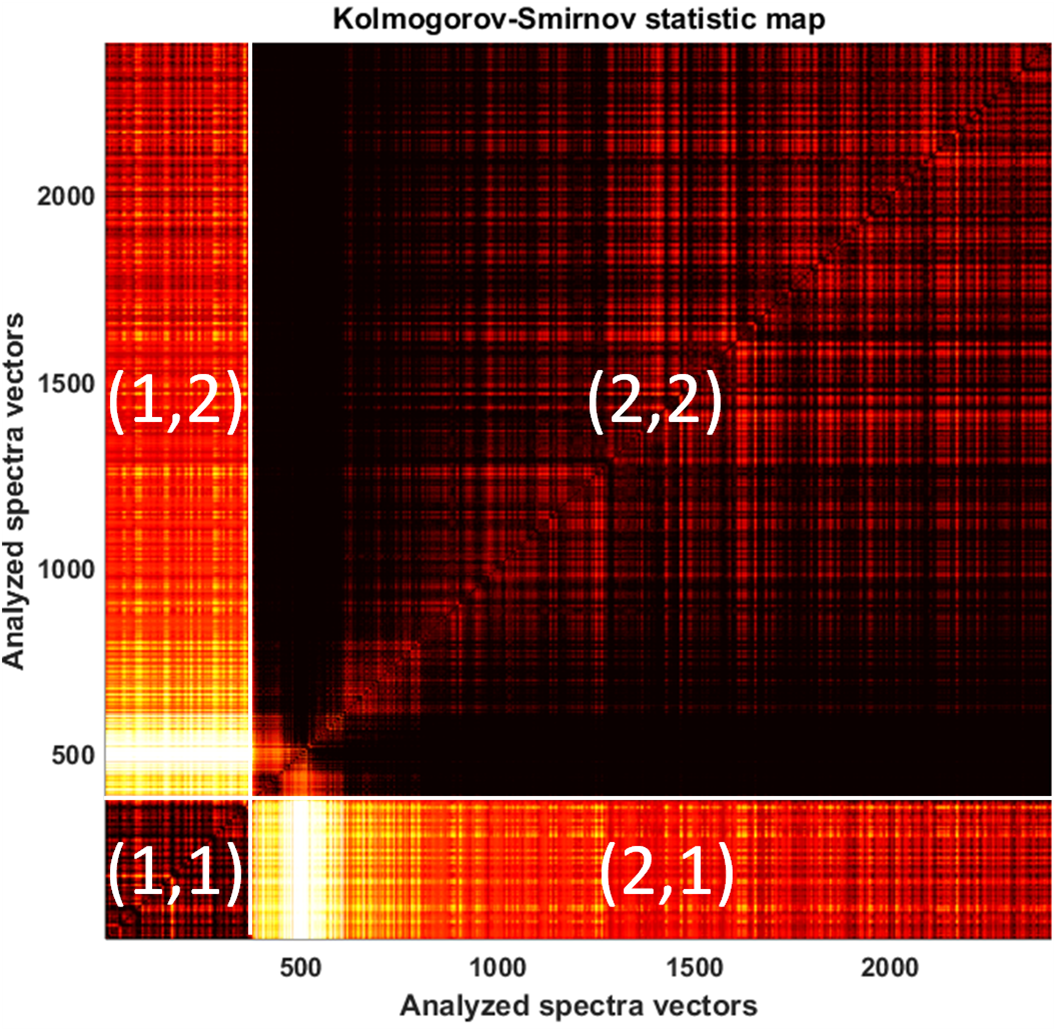
\includegraphics[width = 0.8\textwidth]{figs/map2.png}
\caption{The map of Kolmogorov-Smirnov statistic.}
\label{fig: map}
\end{figure}

Hence, in the next step one-dimensional sum of the map is calculated (see Fig. \ref{fig: duty}). Since the processes share virtually no similarities, one can expect certain behavior of the sum values of particular groups of KS map columns:

\begin{itemize}
\item \textbf{Group regarding process 1 (columns of areas (1,x)):} relatively low energy of the signal. KS statistic values will be low when comparing process 1 to itself, high when the impact occurs and medium and decreasing while the energy damps;
\item \textbf{Group regarding process 2 (columns of areas (2,x)):} relatively high energy. KS statistic values will be low when comparing process 2 to itself, and medium to high when comparing it to process 1.
\end{itemize}

\begin{figure}[!ht]
\centering
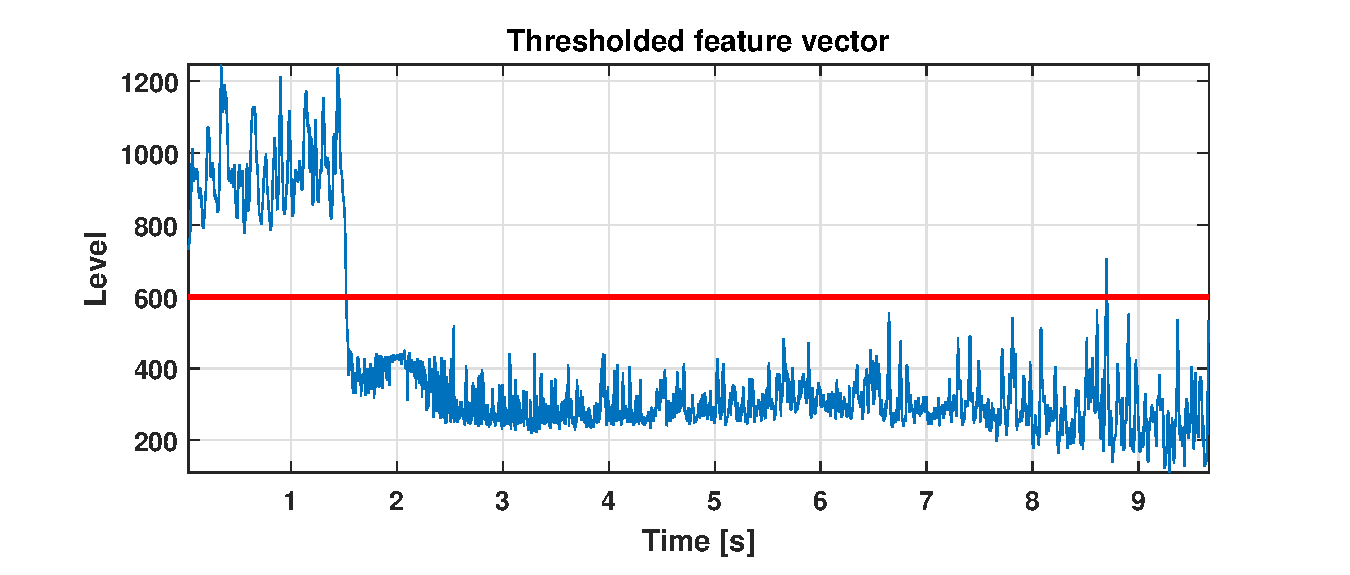
\includegraphics[width = 0.75\textwidth]{figs/duty}
\caption{Feature vector as a result of map integration}
\label{fig: duty}
\end{figure}

To be able to segment out the processes, obtained feature vector is thresholded using central point of histogram as described before (see Fig \ref{fig: hist}). It provided the timestamp of 1.524 seconds, which matches the expert-indicated point exactly, and performs with better precision than STA/LTA method (comparing quotient of a signal under a specific characteristic function in short and long windows \cite{allen1978automatic}). 

\begin{figure}[!ht]
\centering
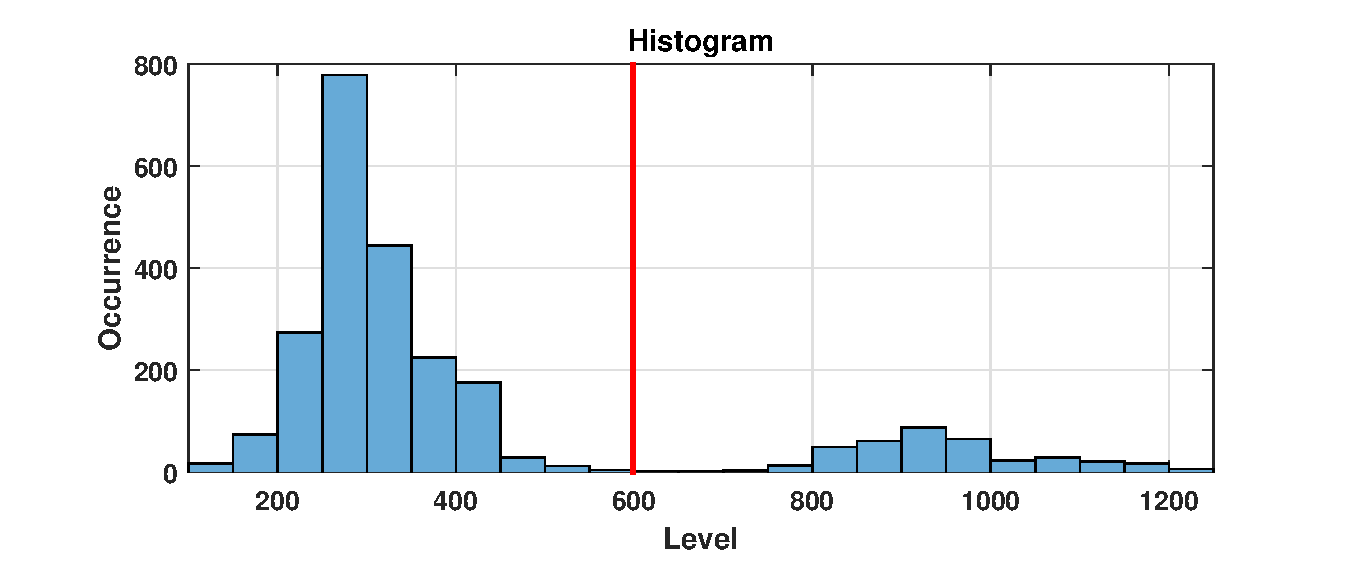
\includegraphics[width = 0.75\textwidth]{figs/hist}
\caption{Histogram of feature vector}
\label{fig: hist}
\end{figure}



\begin{figure}[!ht]
\centering
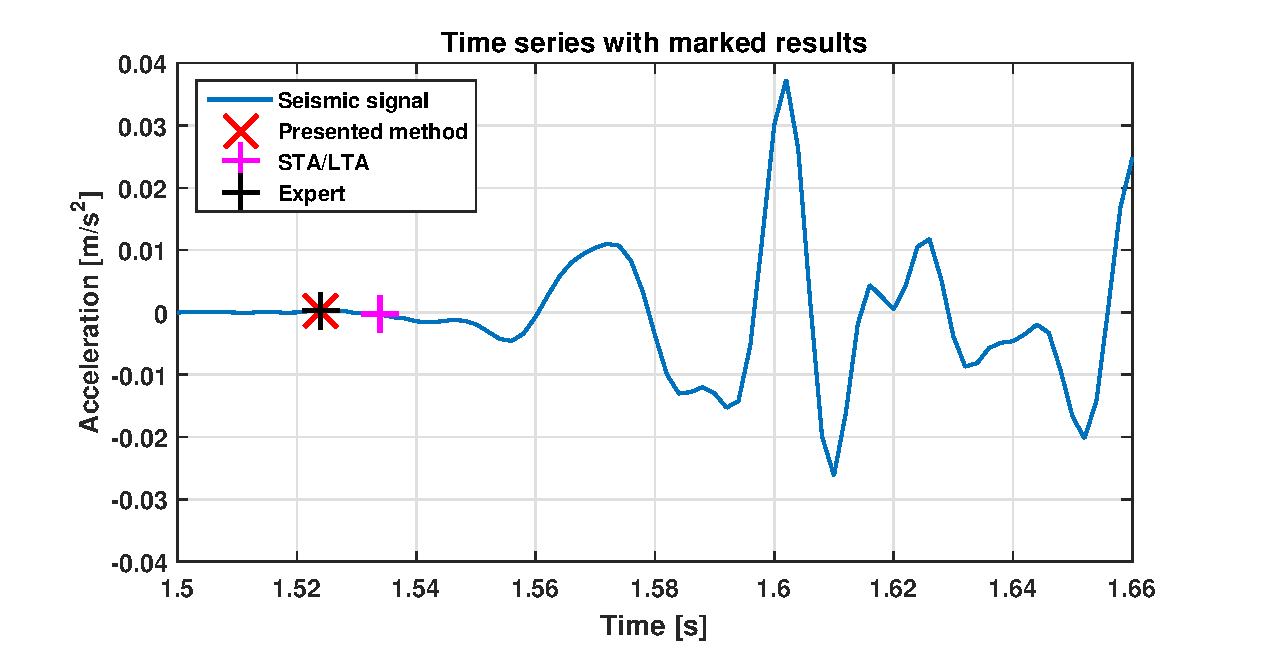
\includegraphics[width = 0.8\textwidth]{figs/final}
\caption{Raw data with marked results of expert, STA/LTA and presented method. Obtained results: 1.524s, 1.532s, 1.524s respectively.}
\label{fig: final}
\end{figure}

\section{Conclusion}

In this article authors present novel approach to P-wave arrival detection in seismic vibration data. Method is based on segmentation of the feature vector constructed from KS statistic map. Entries of the map are KS statistic values that are results of performing KS test on pairs of spectra vectors of signal spectrogram. As a result, algorithm is capable of detection of the P-wave arrival. Presented method produces results consistent with the points indicated manually by seismic experts from the mine and better than commonly used LTA/STA algorithm. Important issue is that the method is automatic and data-driven.

\bibliography{mybibfile}
% end of file template.tex
\end{document}


